%\documentclass[handout]{beamer}
\documentclass{beamer}
%\usepackage{beamerthemesplit}
%\usepackage{logicthemelive}
\usepackage{cite}
\usepackage{enumitem}
\usepackage{pgf}
\usepackage{tikz}
\usepackage{graphicx}
\usepackage{datatool}
\usepackage{dataplot}
\usepackage{xcolor}
\usetikzlibrary{calc,through,decorations.pathmorphing}
\usetikzlibrary{decorations.text}
\usetikzlibrary{trees}
\usetikzlibrary{fit}
\usetikzlibrary{backgrounds}
\usetikzlibrary{positioning}
\usetikzlibrary{shapes,arrows}
\usetikzlibrary{shadows}
\usetikzlibrary{calendar}
%\usepackage[cmex10]{amsmath}
%\usepackage{array}
\usepackage{ctable}
\usepackage{dcolumn}
\usepackage{mdwmath}
\usepackage{mdwtab}
\usepackage{setspace}
\usepackage{fancyhdr}
%\usepackage{electComp}
%\usepackage{amsmath}

\title[Options for improved loss modelling in the New Zealand Electricity Market]{\Large Options for improved loss modelling in the New Zealand Electricity Market}
%\author{Dr David Hume}
%\subtitle{\tiny EEA Conference - 23rd June, 2011} % (optional)
%\author[David Hume]{\normalsize David Hume \\ \tiny {\texttt{david.hume@ea.govt.nz}} \\ \tiny Electricity Authority of New Zealand}
%\institute{\tiny Electricity Authority of New Zealand}
\date{}



\begin{document}

\frame{\titlepage}


%\frame{\tableofcontents}

\section[Effect of power factor on power transfer -- thermal limits]{Effect of power factor on power transfer -- thermal limits}

 
\frame{
 \frametitle{Loss segment approximation -- 2 segments}
\vspace{-10mm}
\begin{center}
\include{default_2}
\end{center}
}

\frame{
 \frametitle{Loss segment approximation -- 3 segments}
\vspace{-10mm}
\begin{center}
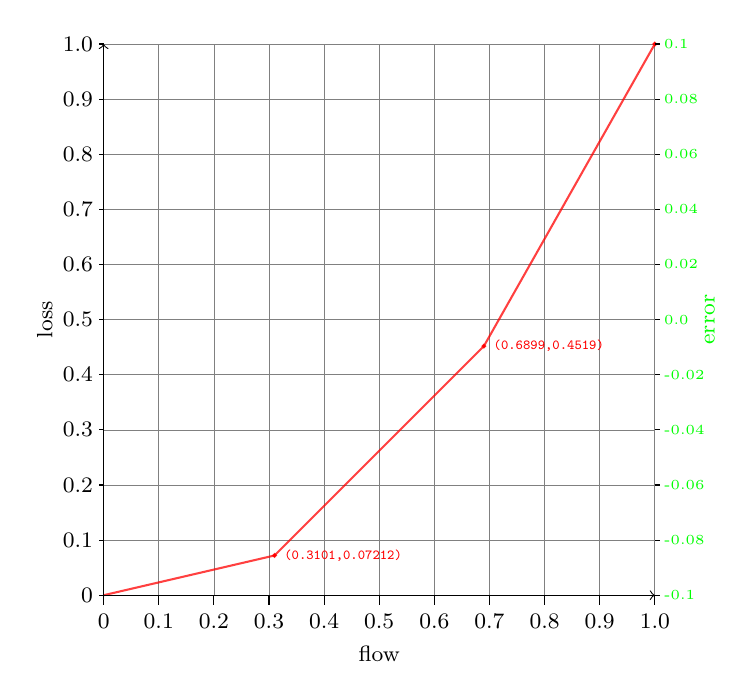
\begin{tikzpicture}[xscale=7.0,yscale=7.0]
\draw [help lines,step=0.1] (0,0) grid (1,1);
\draw[line width=0.5pt,color=black] plot file {default_3_XY.dat};
\coordinate (oneone) at (1,1);
\filldraw [red,draw opacity=0.75] (oneone) circle (0.1pt);
\coordinate (bk1) at (0,0);
\coordinate (bk2) at (0.31009,0.072116);
\coordinate (bk3) at (0.68989,0.45191);
\coordinate (bk4) at (1,1);
\filldraw [red,draw opacity=0.75] (bk2) circle (0.1pt) node[right] {\tiny \texttt{(0.3101,0.07212)}};
\filldraw [red,draw opacity=0.75] (bk3) circle (0.1pt) node[right] {\tiny \texttt{(0.6899,0.4519)}};
\draw[line width=0.75pt,color=red,draw opacity=0.75] (bk1) -- (bk2); 
\draw[line width=0.75pt,color=red,draw opacity=0.75] (bk2) -- (bk3); 
\draw[line width=0.75pt,color=red,draw opacity=0.75] (bk3) -- (bk4); 
\draw[->] (0,0) -- node[midway,yshift=-0.75cm] {\footnotesize flow} (1,0);
\draw[->] (0,0) -- node[rotate=90,midway,yshift=0.75cm] {\footnotesize loss} (0,1) ;
\foreach \x/\xtext in {0,0.1,0.2,0.3,0.4,0.5,0.6,0.7,0.8,0.9,1.0}
\draw (\x cm,0pt) -- (\x cm,-0.5pt) node[anchor=north] {\footnotesize \xtext};
\foreach \y/\ytext in {0,0.1,0.2,0.3,0.4,0.5,0.6,0.7,0.8,0.9,1.0}
\draw (0.0pt,\y cm) -- (-0.25pt,\y cm) node[anchor=east,xshift=0.5mm] {\footnotesize \ytext};
\draw[line width=0.5pt,color=green,draw opacity=0.75] plot file {default_3_err.dat};
\foreach \y/\ytext in {0/-0.1,0.1/-0.08,0.2/-0.06,0.3/-0.04,0.4/-0.02,0.5/0.0,0.6/0.02,0.7/0.04,0.8/0.06,0.9/0.08,1.0/0.1}
\draw (1cm,\y cm) -- (1.01cm,\y cm) node[anchor=west,xshift=-0.75mm] {\tiny \textcolor{green}{\ytext}};
\node[rotate=90] at (1.1,0.5) {\footnotesize \textcolor{green}{error}};
\end{tikzpicture}

\end{center}
}

\frame{
 \frametitle{Loss segment approximation -- 4 segments}
\vspace{-10mm}
\begin{center}
\include{default_4}
\end{center}
}

\frame{
 \frametitle{Loss segment approximation - 5 segments}
\vspace{-10mm}
\begin{center}
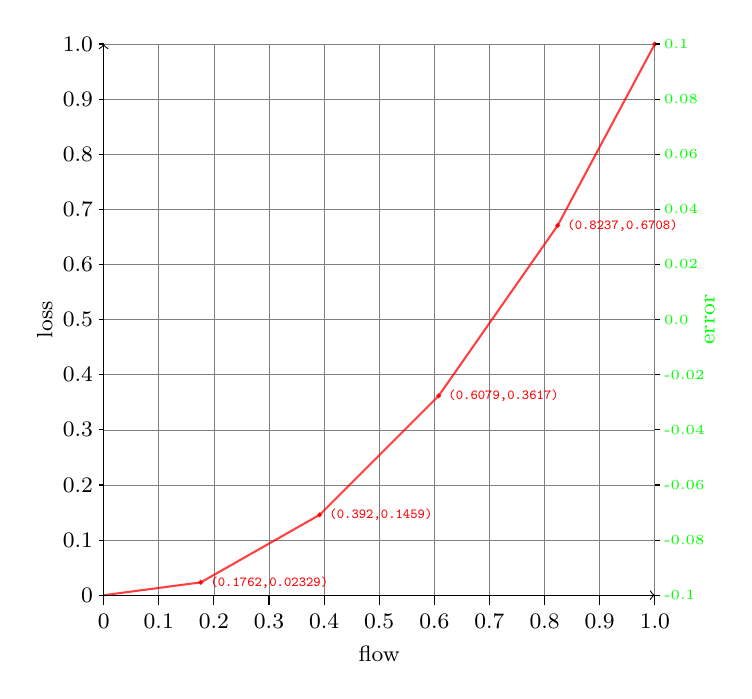
\begin{tikzpicture}[xscale=7.0,yscale=7.0]
\draw [help lines,step=0.1] (0,0) grid (1,1);
\draw[line width=0.5pt,color=black] plot file {default_5_XY.dat};
\coordinate (oneone) at (1,1);
\filldraw [red,draw opacity=0.75] (oneone) circle (0.1pt);
\coordinate (bk1) at (0,0);
\coordinate (bk2) at (0.17621,0.023287);
\coordinate (bk3) at (0.39202,0.14592);
\coordinate (bk4) at (0.60787,0.36174);
\coordinate (bk5) at (0.82374,0.67078);
\coordinate (bk6) at (1,1);
\filldraw [red,draw opacity=0.75] (bk2) circle (0.1pt) node[right] {\tiny \texttt{(0.1762,0.02329)}};
\filldraw [red,draw opacity=0.75] (bk3) circle (0.1pt) node[right] {\tiny \texttt{(0.392,0.1459)}};
\filldraw [red,draw opacity=0.75] (bk4) circle (0.1pt) node[right] {\tiny \texttt{(0.6079,0.3617)}};
\filldraw [red,draw opacity=0.75] (bk5) circle (0.1pt) node[right] {\tiny \texttt{(0.8237,0.6708)}};
\draw[line width=0.75pt,color=red,draw opacity=0.75] (bk1) -- (bk2); 
\draw[line width=0.75pt,color=red,draw opacity=0.75] (bk2) -- (bk3); 
\draw[line width=0.75pt,color=red,draw opacity=0.75] (bk3) -- (bk4); 
\draw[line width=0.75pt,color=red,draw opacity=0.75] (bk4) -- (bk5); 
\draw[line width=0.75pt,color=red,draw opacity=0.75] (bk5) -- (bk6); 
\draw[->] (0,0) -- node[midway,yshift=-0.75cm] {\footnotesize flow} (1,0);
\draw[->] (0,0) -- node[rotate=90,midway,yshift=0.75cm] {\footnotesize loss} (0,1) ;
\foreach \x/\xtext in {0,0.1,0.2,0.3,0.4,0.5,0.6,0.7,0.8,0.9,1.0}
\draw (\x cm,0pt) -- (\x cm,-0.5pt) node[anchor=north] {\footnotesize \xtext};
\foreach \y/\ytext in {0,0.1,0.2,0.3,0.4,0.5,0.6,0.7,0.8,0.9,1.0}
\draw (0.0pt,\y cm) -- (-0.25pt,\y cm) node[anchor=east,xshift=0.5mm] {\footnotesize \ytext};
\draw[line width=0.5pt,color=green,draw opacity=0.75] plot file {default_5_err.dat};
\foreach \y/\ytext in {0/-0.1,0.1/-0.08,0.2/-0.06,0.3/-0.04,0.4/-0.02,0.5/0.0,0.6/0.02,0.7/0.04,0.8/0.06,0.9/0.08,1.0/0.1}
\draw (1cm,\y cm) -- (1.01cm,\y cm) node[anchor=west,xshift=-0.75mm] {\tiny \textcolor{green}{\ytext}};
\node[rotate=90] at (1.1,0.5) {\footnotesize \textcolor{green}{error}};
\end{tikzpicture}

\end{center}
}

\frame{
 \frametitle{Loss segment approximation - 6 segments}
\vspace{-10mm}

\begin{center}
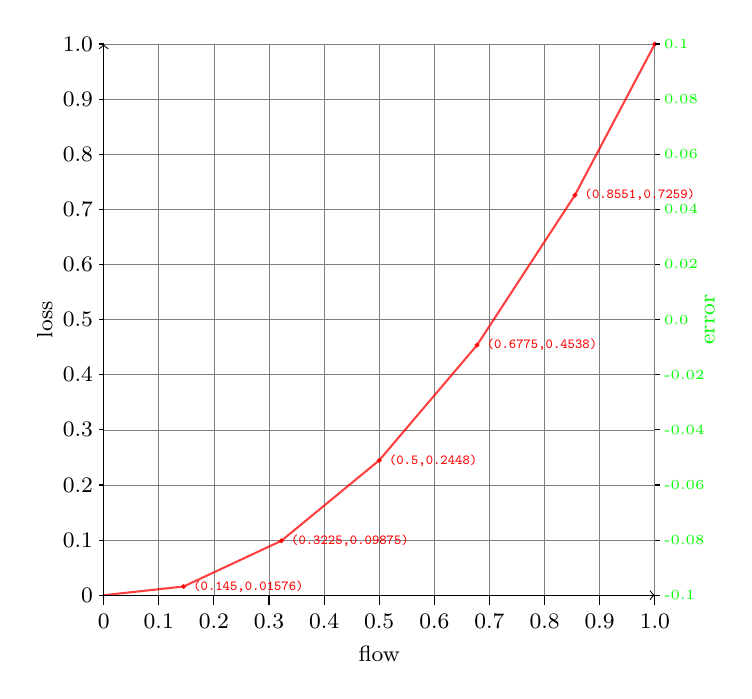
\begin{tikzpicture}[xscale=7.0,yscale=7.0]
\draw [help lines,step=0.1] (0,0) grid (1,1);
\draw[line width=0.5pt,color=black] plot file {default_6_XY.dat};
\coordinate (oneone) at (1,1);
\filldraw [red,draw opacity=0.75] (oneone) circle (0.1pt);
\coordinate (bk1) at (0,0);
\coordinate (bk2) at (0.14497,0.015762);
\coordinate (bk3) at (0.3225,0.098752);
\coordinate (bk4) at (0.50002,0.24477);
\coordinate (bk5) at (0.67754,0.45381);
\coordinate (bk6) at (0.85506,0.72587);
\coordinate (bk7) at (1,1);
\filldraw [red,draw opacity=0.75] (bk2) circle (0.1pt) node[right] {\tiny \texttt{(0.145,0.01576)}};
\filldraw [red,draw opacity=0.75] (bk3) circle (0.1pt) node[right] {\tiny \texttt{(0.3225,0.09875)}};
\filldraw [red,draw opacity=0.75] (bk4) circle (0.1pt) node[right] {\tiny \texttt{(0.5,0.2448)}};
\filldraw [red,draw opacity=0.75] (bk5) circle (0.1pt) node[right] {\tiny \texttt{(0.6775,0.4538)}};
\filldraw [red,draw opacity=0.75] (bk6) circle (0.1pt) node[right] {\tiny \texttt{(0.8551,0.7259)}};
\draw[line width=0.75pt,color=red,draw opacity=0.75] (bk1) -- (bk2); 
\draw[line width=0.75pt,color=red,draw opacity=0.75] (bk2) -- (bk3); 
\draw[line width=0.75pt,color=red,draw opacity=0.75] (bk3) -- (bk4); 
\draw[line width=0.75pt,color=red,draw opacity=0.75] (bk4) -- (bk5); 
\draw[line width=0.75pt,color=red,draw opacity=0.75] (bk5) -- (bk6); 
\draw[line width=0.75pt,color=red,draw opacity=0.75] (bk6) -- (bk7); 
\draw[->] (0,0) -- node[midway,yshift=-0.75cm] {\footnotesize flow} (1,0);
\draw[->] (0,0) -- node[rotate=90,midway,yshift=0.75cm] {\footnotesize loss} (0,1) ;
\foreach \x/\xtext in {0,0.1,0.2,0.3,0.4,0.5,0.6,0.7,0.8,0.9,1.0}
\draw (\x cm,0pt) -- (\x cm,-0.5pt) node[anchor=north] {\footnotesize \xtext};
\foreach \y/\ytext in {0,0.1,0.2,0.3,0.4,0.5,0.6,0.7,0.8,0.9,1.0}
\draw (0.0pt,\y cm) -- (-0.25pt,\y cm) node[anchor=east,xshift=0.5mm] {\footnotesize \ytext};
\draw[line width=0.5pt,color=green,draw opacity=0.75] plot file {default_6_err.dat};
\foreach \y/\ytext in {0/-0.1,0.1/-0.08,0.2/-0.06,0.3/-0.04,0.4/-0.02,0.5/0.0,0.6/0.02,0.7/0.04,0.8/0.06,0.9/0.08,1.0/0.1}
\draw (1cm,\y cm) -- (1.01cm,\y cm) node[anchor=west,xshift=-0.75mm] {\tiny \textcolor{green}{\ytext}};
\node[rotate=90] at (1.1,0.5) {\footnotesize \textcolor{green}{error}};
\end{tikzpicture}

\end{center}
}

\section{Weighted with average circuit and transformer usage during 2010} 

\frame{
 \frametitle{Loss segment approximation -- 2 segments}
\vspace{-10mm}
\begin{center}
\include{tall_2}
\end{center}
}

\frame{
 \frametitle{Loss segment approximation -- 3 segments}
\vspace{-10mm}
\begin{center}
\include{tall_3}
\end{center}
}

\frame{
 \frametitle{Loss segment approximation -- 4 segments}
\vspace{-10mm}
\begin{center}
\include{tall_4}
\end{center}
}

\frame{
 \frametitle{Loss segment approximation - 5 segments}
\vspace{-10mm}
\begin{center}
\include{tall_5}
\end{center}
}

\frame{
 \frametitle{Loss segment approximation - 6 segments}
\vspace{-10mm}

\begin{center}
\include{tall_6}
\end{center}
}


\section{Transmission circuits loss segments (weighted with average circuit usage during 2010)} 

\frame{
 \frametitle{Loss segment approximation -- 2 segments}
\vspace{-10mm}
\begin{center}
\include{tcuse_2}
\end{center}
}

\frame{
 \frametitle{Loss segment approximation -- 3 segments}
\vspace{-10mm}
\begin{center}
\include{tcuse_3}
\end{center}
}

\frame{
 \frametitle{Loss segment approximation -- 4 segments}
\vspace{-10mm}
\begin{center}
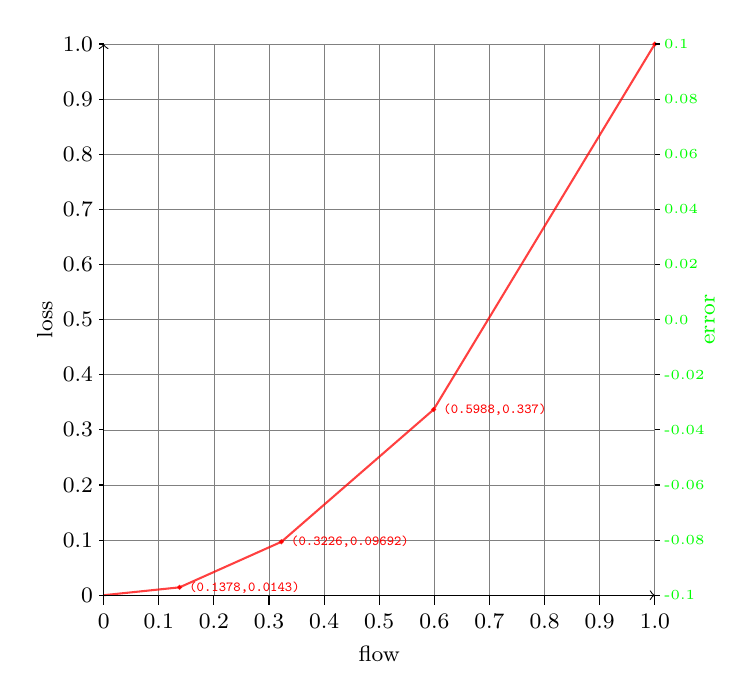
\begin{tikzpicture}[xscale=7.0,yscale=7.0]
\draw [help lines,step=0.1] (0,0) grid (1,1);
\filldraw[line width=0.5pt,color=blue!25!white,draw opacity=0.15,fill opacity = 0.5] plot file {tcuse_4_hg.dat};
\draw[line width=0.5pt,color=black] plot file {tcuse_4_XY.dat};
\coordinate (oneone) at (1,1);
\filldraw [red,draw opacity=0.75] (oneone) circle (0.1pt);
\coordinate (bk1) at (0,0);
\coordinate (bk2) at (0.13781,0.014302);
\coordinate (bk3) at (0.32256,0.096921);
\coordinate (bk4) at (0.59881,0.33698);
\coordinate (bk5) at (1,1);
\filldraw [red,draw opacity=0.75] (bk2) circle (0.1pt) node[right] {\tiny \texttt{(0.1378,0.0143)}};
\filldraw [red,draw opacity=0.75] (bk3) circle (0.1pt) node[right] {\tiny \texttt{(0.3226,0.09692)}};
\filldraw [red,draw opacity=0.75] (bk4) circle (0.1pt) node[right] {\tiny \texttt{(0.5988,0.337)}};
\draw[line width=0.75pt,color=red,draw opacity=0.75] (bk1) -- (bk2); 
\draw[line width=0.75pt,color=red,draw opacity=0.75] (bk2) -- (bk3); 
\draw[line width=0.75pt,color=red,draw opacity=0.75] (bk3) -- (bk4); 
\draw[line width=0.75pt,color=red,draw opacity=0.75] (bk4) -- (bk5); 
\draw[->] (0,0) -- node[midway,yshift=-0.75cm] {\footnotesize flow} (1,0);
\draw[->] (0,0) -- node[rotate=90,midway,yshift=0.75cm] {\footnotesize loss} (0,1) ;
\foreach \x/\xtext in {0,0.1,0.2,0.3,0.4,0.5,0.6,0.7,0.8,0.9,1.0}
\draw (\x cm,0pt) -- (\x cm,-0.5pt) node[anchor=north] {\footnotesize \xtext};
\foreach \y/\ytext in {0,0.1,0.2,0.3,0.4,0.5,0.6,0.7,0.8,0.9,1.0}
\draw (0.0pt,\y cm) -- (-0.25pt,\y cm) node[anchor=east,xshift=0.5mm] {\footnotesize \ytext};
\draw[line width=0.5pt,color=green,draw opacity=0.75] plot file {tcuse_4_err.dat};
\foreach \y/\ytext in {0/-0.1,0.1/-0.08,0.2/-0.06,0.3/-0.04,0.4/-0.02,0.5/0.0,0.6/0.02,0.7/0.04,0.8/0.06,0.9/0.08,1.0/0.1}
\draw (1cm,\y cm) -- (1.01cm,\y cm) node[anchor=west,xshift=-0.75mm] {\tiny \textcolor{green}{\ytext}};
\node[rotate=90] at (1.1,0.5) {\footnotesize \textcolor{green}{error}};
\end{tikzpicture}

\end{center}
}

\frame{
 \frametitle{Loss segment approximation - 5 segments}
\vspace{-10mm}
\begin{center}
\include{tcuse_5}
\end{center}
}

\frame{
 \frametitle{Loss segment approximation - 6 segments}
\vspace{-10mm}

\begin{center}
\include{tcuse_6}
\end{center}
}


\section{Transformer circuits loss segments (weighted with average circuit usage during 2010)} 

\frame{
 \frametitle{Loss segment approximation -- 2 segments}
\vspace{-10mm}
\begin{center}
\include{txuse_2}
\end{center}
}

\frame{
 \frametitle{Loss segment approximation -- 3 segments}
\vspace{-10mm}
\begin{center}
\include{txuse_3}
\end{center}
}

\frame{
 \frametitle{Loss segment approximation -- 4 segments}
\vspace{-10mm}
\begin{center}
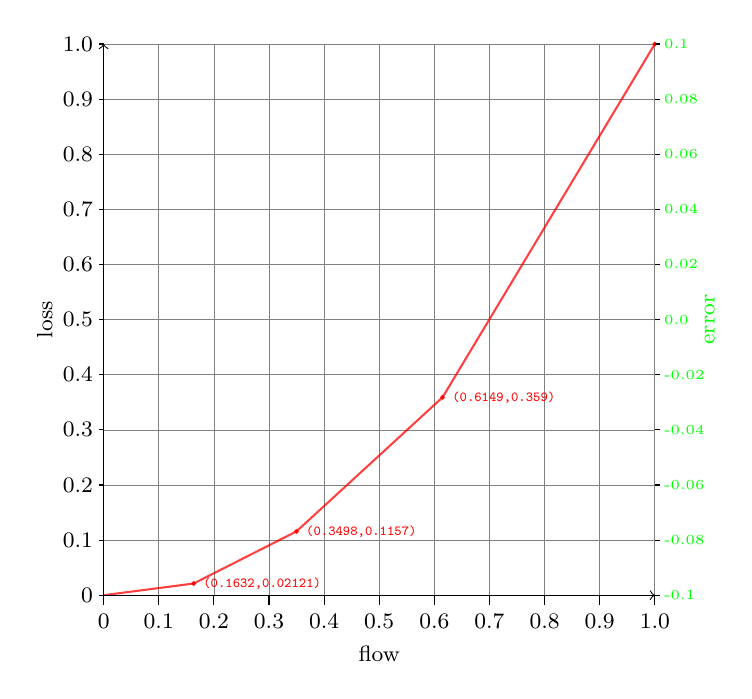
\begin{tikzpicture}[xscale=7.0,yscale=7.0]
\draw [help lines,step=0.1] (0,0) grid (1,1);
\filldraw[line width=0.5pt,color=blue!25!white,draw opacity=0.15,fill opacity = 0.5] plot file {txuse_4_hg.dat};
\draw[line width=0.5pt,color=black] plot file {txuse_4_XY.dat};
\coordinate (oneone) at (1,1);
\filldraw [red,draw opacity=0.75] (oneone) circle (0.1pt);
\coordinate (bk1) at (0,0);
\coordinate (bk2) at (0.16322,0.021208);
\coordinate (bk3) at (0.34979,0.11569);
\coordinate (bk4) at (0.6149,0.35903);
\coordinate (bk5) at (1,1);
\filldraw [red,draw opacity=0.75] (bk2) circle (0.1pt) node[right] {\tiny \texttt{(0.1632,0.02121)}};
\filldraw [red,draw opacity=0.75] (bk3) circle (0.1pt) node[right] {\tiny \texttt{(0.3498,0.1157)}};
\filldraw [red,draw opacity=0.75] (bk4) circle (0.1pt) node[right] {\tiny \texttt{(0.6149,0.359)}};
\draw[line width=0.75pt,color=red,draw opacity=0.75] (bk1) -- (bk2); 
\draw[line width=0.75pt,color=red,draw opacity=0.75] (bk2) -- (bk3); 
\draw[line width=0.75pt,color=red,draw opacity=0.75] (bk3) -- (bk4); 
\draw[line width=0.75pt,color=red,draw opacity=0.75] (bk4) -- (bk5); 
\draw[->] (0,0) -- node[midway,yshift=-0.75cm] {\footnotesize flow} (1,0);
\draw[->] (0,0) -- node[rotate=90,midway,yshift=0.75cm] {\footnotesize loss} (0,1) ;
\foreach \x/\xtext in {0,0.1,0.2,0.3,0.4,0.5,0.6,0.7,0.8,0.9,1.0}
\draw (\x cm,0pt) -- (\x cm,-0.5pt) node[anchor=north] {\footnotesize \xtext};
\foreach \y/\ytext in {0,0.1,0.2,0.3,0.4,0.5,0.6,0.7,0.8,0.9,1.0}
\draw (0.0pt,\y cm) -- (-0.25pt,\y cm) node[anchor=east,xshift=0.5mm] {\footnotesize \ytext};
\draw[line width=0.5pt,color=green,draw opacity=0.75] plot file {txuse_4_err.dat};
\foreach \y/\ytext in {0/-0.1,0.1/-0.08,0.2/-0.06,0.3/-0.04,0.4/-0.02,0.5/0.0,0.6/0.02,0.7/0.04,0.8/0.06,0.9/0.08,1.0/0.1}
\draw (1cm,\y cm) -- (1.01cm,\y cm) node[anchor=west,xshift=-0.75mm] {\tiny \textcolor{green}{\ytext}};
\node[rotate=90] at (1.1,0.5) {\footnotesize \textcolor{green}{error}};
\end{tikzpicture}

\end{center}
}

\frame{
 \frametitle{Loss segment approximation - 5 segments}
\vspace{-10mm}
\begin{center}
\include{txuse_5}
\end{center}
}

\frame{
 \frametitle{Loss segment approximation - 6 segments}
\vspace{-10mm}

\begin{center}
\include{txuse_6}
\end{center}
}



\end{document}
    